\documentclass[11pt,a4paper]{article}

% NAVISense Vest report template
% Recommended compiler: XeLaTeX
% Also compiles with pdfLaTeX using fallback fonts.

\usepackage[a4paper,margin=22mm,headheight=18pt,headsep=12pt,footskip=18pt]{geometry}
\usepackage{iftex}
\ifPDFTeX
  \usepackage[T1]{fontenc}
  \usepackage[utf8]{inputenc}
  \usepackage{helvet}
\else
  \usepackage{fontspec}
\fi
\usepackage{xcolor}
\usepackage{graphicx}
\usepackage{tikz}
\usepackage[most]{tcolorbox}
\usepackage{titlesec}
\usepackage{enumitem}
\usepackage{tabularx}
\usepackage{array}
\usepackage{booktabs}
\usepackage{colortbl}
\usepackage{fancyhdr}
\usepackage{lastpage}
\usepackage{hyperref}
\usepackage{microtype}
\usepackage{eso-pic}

\graphicspath{{assets/}}
\usetikzlibrary{calc}

% ---------- Brand Tokens ----------
\definecolor{NaviBg}{HTML}{020326}
\definecolor{NaviBgSoft}{HTML}{050816}
\definecolor{NaviBlue}{HTML}{031B70}
\definecolor{NaviIndigo}{HTML}{2F2C8F}
\definecolor{NaviCyan}{HTML}{5FA9E8}
\definecolor{NaviCyanStrong}{HTML}{1C7CC7}
\definecolor{NaviPurple}{HTML}{A88FFF}
\definecolor{NaviGold}{HTML}{FFD966}
\definecolor{NaviGreen}{HTML}{34D399}
\definecolor{NaviText}{HTML}{F8FAFC}
\definecolor{NaviMuted}{HTML}{C9D2E2}
\definecolor{NaviLine}{HTML}{36508E}
\definecolor{NaviCard}{HTML}{172056}
\definecolor{NaviCardSoft}{HTML}{0E1646}

\pagecolor{NaviBg}
\color{NaviText}
\linespread{1.045}

% ---------- Fonts ----------
\ifPDFTeX
  \renewcommand{\familydefault}{\sfdefault}
  \newcommand{\DisplayFont}{\sffamily}
\else
  \IfFontExistsTF{Inter}
    {\setsansfont{Inter}}
    {\setsansfont{TeX Gyre Heros}}

  \IfFontExistsTF{Syne}
    {\newfontfamily\DisplayFont{Syne}}
    {\newfontfamily\DisplayFont{TeX Gyre Heros}}

  \renewcommand{\familydefault}{\sfdefault}
\fi

% ---------- Report Metadata ----------
\newcommand{\ReportTitle}{Report Title Goes Here}
\newcommand{\ReportSubtitle}{Short report subtitle or one-line context.}
\newcommand{\ReportCategory}{Development}
\newcommand{\ReportAuthor}{NAVISense Team}
\newcommand{\ReportDate}{April 2026}
\newcommand{\ReportVersion}{v1.0}
\newcommand{\ReportStatus}{In progress}

% ---------- Page Background ----------
\newcommand{\NaviBackground}{%
  
\begin{tikzpicture}[remember picture,overlay]
    \fill[NaviBg] (current page.south west) rectangle (current page.north east);

    \path[fill=NaviBlue,opacity=0.46]
      (current page.south west) rectangle ($(current page.north east)+(0,0)$);

    \shade[inner color=NaviCyan,outer color=NaviBg,opacity=0.145]
      ($(current page.south west)+(26mm,45mm)$) circle (64mm);
    \shade[inner color=NaviPurple,outer color=NaviBg,opacity=0.13]
      ($(current page.north west)+(48mm,-48mm)$) circle (72mm);
    \shade[inner color=NaviIndigo,outer color=NaviBg,opacity=0.145]
      ($(current page.north east)+(-36mm,-76mm)$) circle (78mm);

    \draw[step=10mm,NaviCyan,opacity=0.030,line width=0.22pt]
      (current page.south west) grid (current page.north east);
  \end{tikzpicture}%
}

\AddToShipoutPictureBG{\NaviBackground}

% ---------- Hyperlinks ----------
\hypersetup{
  colorlinks=true,
  linkcolor=NaviCyan,
  urlcolor=NaviCyan,
  citecolor=NaviPurple,
  pdfauthor={NAVISense Team},
  pdftitle={NAVISense Report}
}

% ---------- Headings ----------
\titleformat{\section}
  {\DisplayFont\large\bfseries\color{NaviText}}
  {}
  {0pt}
  {\color{NaviCyan}\thesection\hspace{0.65em}\color{NaviText}}
  [\vspace{4pt}{\color{NaviCyan!82}\titlerule[0.48pt]}]

\titleformat{\subsection}
  {\DisplayFont\normalsize\bfseries\color{NaviCyan}}
  {}
  {0pt}
  {\thesubsection\hspace{0.6em}}

\titlespacing*{\section}{0pt}{18pt}{11pt}
\titlespacing*{\subsection}{0pt}{12pt}{6pt}

\setlist[itemize]{
  leftmargin=18pt,
  itemsep=4pt,
  topsep=4pt,
  label=\textcolor{NaviCyan}{\small\textbullet}
}

\setlength{\parindent}{0pt}
\setlength{\parskip}{6.5pt}
\renewcommand{\arraystretch}{1.25}
\arrayrulecolor{NaviLine}
\renewcommand{\tabularxcolumn}[1]{m{#1}}
\newcommand{\NaviTableCellStart}{\raggedright\arraybackslash\strut}
\newcolumntype{L}[1]{>{\NaviTableCellStart}m{#1}}
\newcolumntype{B}[1]{>{\bfseries\color{NaviCyan}\NaviTableCellStart}m{#1}}
\newcolumntype{Y}{>{\NaviTableCellStart}X}

% ---------- Header / Footer ----------
\pagestyle{fancy}
\fancyhf{}
\renewcommand{\headrulewidth}{0pt}
\renewcommand{\footrulewidth}{0pt}
\fancyhead[L]{%
  \raisebox{-2pt}{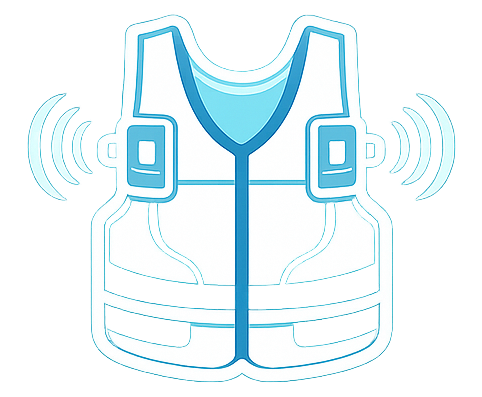
\includegraphics[height=13pt]{vesticon.png}}\hspace{7pt}%
  {\footnotesize\color{NaviMuted}\ReportCategory}
}
\fancyhead[R]{\footnotesize\color{NaviMuted}\ReportDate}
\fancyfoot[L]{\footnotesize\color{NaviMuted}NAVISense Vest}
\fancyfoot[R]{\footnotesize\color{NaviMuted}\thepage\ /\ \pageref*{LastPage}}

% ---------- Reusable Components ----------
\newcommand{\NaviTag}[2][NaviCyan]{%
  \tikz[baseline=(tag.base)]{
    \node[
      inner xsep=7pt,
      inner ysep=3pt,
      rounded corners=7pt,
      draw=#1!40,
      fill=#1!15,
      text=#1,
      font=\scriptsize\bfseries
    ] (tag) {\MakeUppercase{#2}};
  }%
}

\newcommand{\NaviMetric}[3]{%
  \begin{tcolorbox}[
    enhanced,
    colback=NaviCard!76,
    colframe=NaviCyan!18,
    boxrule=0.4pt,
    arc=7pt,
    left=10pt,
    right=10pt,
    top=8pt,
    bottom=8pt,
    height=28mm,
    borderline north={0.3pt}{0pt}{white!10}
  ]
    {\DisplayFont\Large\bfseries\color{NaviCyan!92}#1}\par
    {\scriptsize\bfseries\color{NaviMuted}\MakeUppercase{#2}}\par
    {\footnotesize\color{NaviText!92}#3}
  \end{tcolorbox}
}

\newtcolorbox{NaviGlassBox}[1][]{
  enhanced,
  breakable,
  colback=NaviCard!68,
  colframe=NaviCyan!14,
  boxrule=0.38pt,
  arc=8pt,
  left=12pt,
  right=12pt,
  top=11pt,
  bottom=11pt,
  borderline north={0.3pt}{0pt}{white!11},
  #1
}

\newtcolorbox{NaviAccentBox}[2][]{
  enhanced,
  breakable,
  title={#2},
  coltitle=NaviText,
  fonttitle=\DisplayFont\bfseries,
  colback=NaviCardSoft!82,
  colframe=NaviPurple!22,
  boxrule=0.42pt,
  arc=8pt,
  left=12pt,
  right=12pt,
  top=10pt,
  bottom=11pt,
  attach boxed title to top left={xshift=10pt,yshift=-3pt},
  boxed title style={
    colback=NaviPurple!14,
    colframe=NaviPurple!24,
    arc=7pt,
    boxrule=0.4pt,
    left=7pt,
    right=7pt,
    top=3pt,
    bottom=3pt
  },
  #1
}

\newtcolorbox{NaviLeadBox}[1][]{
  enhanced,
  breakable,
  colback=NaviBgSoft!54,
  colframe=NaviCyan!24,
  boxrule=0.35pt,
  arc=6pt,
  left=13pt,
  right=13pt,
  top=11pt,
  bottom=11pt,
  borderline west={1.2pt}{0pt}{NaviCyan!78},
  #1
}

\newcommand{\NaviSectionNote}[2]{%
  \vspace{2pt}
  {\DisplayFont\bfseries\color{NaviCyan}#1}\par
  {\color{NaviMuted}#2}
  \vspace{4pt}
}

\newcommand{\NaviMilestone}[4]{%
  \begin{NaviGlassBox}
    \NaviTag[#1]{#2}\hfill{\footnotesize\color{NaviMuted}#3}\par
    \vspace{3pt}
    {\color{NaviText}#4}
  \end{NaviGlassBox}
}

\newcommand{\NaviDivider}{%
  \vspace{6pt}
  {\color{NaviLine}\hrule height 0.45pt}
  \vspace{8pt}
}

\newcommand{\NaviMetaLabel}[1]{%
  {\scriptsize\bfseries\color{NaviCyan}\MakeUppercase{#1}}%
}

\newcommand{\NaviMetaValue}[1]{%
  {\small\color{NaviText}#1}%
}

% ---------- Cover ----------
\newcommand{\MakeNaviCover}{%
  \thispagestyle{empty}

  \vspace*{10mm}
  \noindent\begin{minipage}{0.48\textwidth}
    
\includegraphics[width=39mm]{navisense-logo.png}\par
  \end{minipage}
  \hfill
  \begin{minipage}{0.46\textwidth}
    \raggedleft
    {\scriptsize\bfseries\color{NaviCyan}\MakeUppercase{Full report}}\par
    \vspace{2mm}
    {\footnotesize\color{NaviMuted}\ReportDate}\par
    {\footnotesize\color{NaviMuted}\ReportAuthor}\par
    \vspace{3mm}
    {\color{NaviCyan!70}\rule{30mm}{0.45pt}}
  \end{minipage}

  \vspace{30mm}
  \noindent\begin{minipage}{\textwidth}
    {\DisplayFont\fontsize{31}{34}\selectfont\bfseries\color{NaviText}\ReportTitle\par}
    \vspace{7mm}
    {\large\color{NaviMuted!94}\ReportSubtitle\par}
  \end{minipage}

  \vspace{13mm}
  {\color{NaviCyan!76}\hrule height 0.45pt}
  \vspace{3mm}
  \noindent\begin{tabularx}{\textwidth}{@{}X X X@{}}
    \NaviMetaLabel{Category} & \NaviMetaLabel{Status} & \NaviMetaLabel{Version} \\
    \NaviMetaValue{\ReportCategory} & \NaviMetaValue{\ReportStatus} & \NaviMetaValue{\ReportVersion}
  \end{tabularx}
  \vspace{3mm}
  {\color{NaviLine}\hrule height 0.35pt}

  \vfill
  \noindent\begin{minipage}{\textwidth}
    {\DisplayFont\normalsize\bfseries\color{NaviCyan}Executive signal}\par
    \vspace{2mm}
    {\color{NaviMuted!94}
    Use this cover note to frame the report in one sentence: what changed, why it matters,
    and what the reader should take away before reading the details.
    \par}
    \vspace{4mm}
    {\color{NaviCyan!78}\hrule height 0.5pt}
  \end{minipage}
  \clearpage
}

\begin{document}

% Edit these values for each blog report.
\renewcommand{\ReportTitle}{Prototype Development Report}
\renewcommand{\ReportSubtitle}{A focused technical note on progress, decisions, risks, and next steps.}
\renewcommand{\ReportCategory}{Development}
\renewcommand{\ReportAuthor}{NAVISense Team}
\renewcommand{\ReportDate}{April 2026}
\renewcommand{\ReportVersion}{v1.0}
\renewcommand{\ReportStatus}{Draft}

\MakeNaviCover

\section{Executive Summary}
This report summarizes the current state of the NAVISense Vest workstream. Replace this
paragraph with a concise overview of what happened, what changed, and why the update
matters for the project.

\vspace{4pt}
\arrayrulecolor{NaviCyan!48}
\begin{tabularx}{\textwidth}{|B{0.22\textwidth}|Y|}
\hline
Progress & Prototype integration is moving through the active build phase. \\
\hline
Key risks & Power budget and sensor latency require continued validation. \\
\hline
Next focus & Prepare reliable testing sessions with repeatable scenarios. \\
\hline
\end{tabularx}
\arrayrulecolor{NaviLine}

\section{Context}
Explain the background of this report: what triggered the work, what decisions had already
been made, and which part of the system this update covers.

\NaviSectionNote{Useful framing}{Keep this section short. A report should not repeat the
whole project proposal; it should make the current update easy to understand.}

\section{Work Completed}
\begin{itemize}
  \item Replaced this bullet with a concrete task or decision.
  \item Mention the responsible person or subsystem when useful.
  \item Link each completed item to evidence, measurements, screenshots, or diagrams.
\end{itemize}

\section{Technical Notes}
\subsection{Architecture}
Use this subsection for diagrams, component interactions, database/API decisions, firmware
notes, or implementation details.

\NaviSectionNote{Example note}{The vest-to-application communication path should describe
sensor input, embedded processing, data transmission, dashboard storage, and user feedback.}

\subsection{Evidence}
Add measurements, test data, screenshots, or references here.

\begin{center}
\begin{tcolorbox}[
  enhanced,
  width=0.78\textwidth,
  height=42mm,
  colback=NaviCardSoft!58,
  colframe=NaviCyan!14,
  boxrule=0.38pt,
  arc=8pt,
  valign=center,
  halign=center,
  borderline north={0.3pt}{0pt}{white!9}
]
{\color{NaviMuted}Drop an image, chart, circuit capture, or dashboard screenshot here.}
\end{tcolorbox}
\end{center}

\section{Risks and Mitigations}
\arrayrulecolor{NaviCyan!48}
\begin{tabularx}{\textwidth}{|B{0.23\textwidth}|Y|Y|}
\hline
{\bfseries\color{NaviCyan}Risk} & {\bfseries\color{NaviCyan}Impact} & {\bfseries\color{NaviCyan}Mitigation} \\
\hline
Sensor latency & Navigation feedback may feel late or confusing. & Run controlled latency tests and define acceptable thresholds. \\
\hline
Power draw & Battery life may be lower than expected. & Profile current draw by subsystem and prioritize sleep states. \\
\hline
Mechanical comfort & The vest may become uncomfortable over longer use. & Collect user feedback during short fitting sessions. \\
\hline
\end{tabularx}
\arrayrulecolor{NaviLine}

\section{Timeline}
\begin{tabularx}{\textwidth}{@{}B{0.18\textwidth} L{0.22\textwidth} Y@{}}
\toprule
Stage & Period & Description \\
\midrule
Completed & Week 01 & Initial research, component selection, and report framing. \\
In progress & Week 02 & Prototype integration and early validation. \\
Next & Week 03 & Structured testing, evidence collection, and blog publication. \\
\bottomrule
\end{tabularx}

\section{Next Steps}
\begin{itemize}
  \item Define the next measurable deliverable.
  \item Assign owners and deadlines.
  \item Decide what evidence should be collected for the next full report.
\end{itemize}

\section{Appendix}
Use the appendix for raw notes, tables, screenshots, links, or references that are useful
but too detailed for the main narrative.

\end{document}
